% Front half of the capstone report: Abstract, Executive Summary, Introduction, Background, Data, Methodology.
% Numbers come from the shared facts file (as of 2026-11-03). Running or planned experiments use \pending{...}.
% Labels defined here: fig:intuition, tab:phases, tab:datasets, tab:structure, tab:variants.
% Labels used from the back half: app:background.

\section*{Abstract}
\noindent Graph neural networks predict a property of each node by passing information along the edges of a graph. They can fail when the information a node needs sits far away. Message passing squeezes distant signals through narrow bridges in the graph (over-squashing), while global attention spreads its focus over too many nodes (attention dilution). This project asks whether the structure of a graph and the range of a task predict how far a model should be allowed to look. We study large social graphs from SNAP (Twitch, Reddit and the Twitter Higgs-boson network), which existing long-range benchmarks do not cover. We measure over-squashing with excess effective resistance and Jacobian sensitivity, dilution with attention entropy, and task range with a Jacobian-based measure. Our first knob, a blend weight between message passing and attention, was partly undone by learnable normalisation scales, so we replace it with an attention radius $k$. On Twitter Higgs, no graph model beat a features-only baseline when trained on 500-node subgraphs, and a simple check showed that cutting the graph threw away most of the neighbour signal. Full-graph training and planted targets with a known range are running.

\vspace{1in}
\noindent\textit{Keywords:} graph neural networks, social networks, over-squashing, attention dilution, effective resistance, attention radius, task range, graph transformers, semi-synthetic benchmarks

\newpage
\section*{Executive Summary}
Many prediction problems live on networks: will this user become active, is this channel for adults, what does this community talk about. Graph neural networks (GNNs) answer such questions by letting each node collect information from its neighbours. Two designs dominate. Message passing relays information one hop at a time and can lose distant information at bottlenecks. Attention lets a node look at every other node at once, but it can then spread its focus too thin. Practitioners usually train both and keep the winner. We want a rule that says in advance how far a model should look, based on the graph's structure and on how far the task needs to reach.

\textbf{What is done.} We built a tested data pipeline for four large social graphs from SNAP, with checks that no future information leaks into the inputs. We built the models (message passing, three kinds of attention, hybrids and two baselines) and the measurements of over-squashing, dilution and range. We ran two sweeps on the Twitter Higgs graph.

\textbf{What we learned.} First, on large social graphs the standard bottleneck measure, effective resistance, mostly restates node degree, so we use a degree-corrected version (excess resistance). Second, our original knob, a blend weight $\alpha$ between message passing and attention, was partly undone during training by the learnable scales of the normalisation layers. We fixed this and added a cleaner knob, the attention radius $k$. Third, on Higgs no graph model beat a simple model that ignores the graph (test AUROC 0.710 for the simple model on 500-node subgraphs). A direct check explained why: cutting the graph into small pieces for training kept only about a third of the edges and removed most of the useful neighbour signal. On social graphs, subgraph training throws away what the models need.

\textbf{What is pending.} We are now training on the whole graph, sweeping both knobs. We are also building planted targets: real graphs and features with an added signal whose range is known exactly. They let us check that the range measure works and that the best radius follows the task's range. Results of these runs, the phase diagram, a test of graph foundation models and a benchmark release are still to come.

\maintextstart

\section{Introduction}
Graph neural networks are the standard tool for learning on networked data such as social networks, molecules and transport systems. In each setting, the prediction for one node can depend on nodes several steps away. Whether a model can use that distant information depends on how the model moves information around, and the two main designs move it in opposite ways. A message-passing network moves information one edge per layer. A graph transformer lets every node attend to (look at) every other node in a single layer. Hybrid models combine both. There is still no principled way to decide in advance which design, or which mix, a given graph and task need.

\subsection{Problem Statement}
Current practice is trial and error: train a message-passing model, a graph transformer and a hybrid such as GPS \citep{rampasek2022}, then keep the one with the best validation score. This costs several full training runs per task and does not explain why the winner won. The answer also does not transfer, because a score on one graph says little about the next.

The difficulty is that long-range learning can fail for two different reasons. \emph{Over-squashing} happens when information from many distant nodes must squeeze through a few bridge nodes and gets compressed into fixed-size vectors \citep{alon2021,topping2022}. Effective resistance, a measure of how hard it is for two nodes to communicate, bounds this effect \citep{digiovanni2023,black2023}. \emph{Attention dilution} is the opposite failure: when attention covers many nodes and does not concentrate, each relevant node gets only a small share of the focus \citep{xing2024}. A model that reaches further avoids the first problem but invites the second. Benchmarks have not settled which matters when. Well-tuned message-passing models close most of the reported gap to transformers on the Long Range Graph Benchmark \citep{tonshoff2024}, and some of its tasks turn out to need only short-range information \citep{bamberger2025}.

Social graphs make the question sharper. They are large, they have hubs with thousands of followers, and almost every pair of users is joined by a short path. No existing long-range benchmark contains a social graph: LRGB has vision, chemistry and quantum-chemistry graphs \citep{dwivedi2022}, and ECHO has synthetic long-diameter graphs and molecules \citep{miglior2025}. So we do not know whether long-range reasoning matters on social data, or how to tune a model for it.

\subsection{Research Goals}
The project asks one question: \emph{can the structure of a graph and the range of a task predict how far a model's attention should reach?} We answer it with three components.
\begin{enumerate}
\item \textbf{Measurements on trained models.} Jacobian sensitivity against (excess) effective resistance for over-squashing; attention entropy for dilution; and the range measure of \citet{bamberger2025} for how far a model's predictions actually reach.
\item \textbf{Controlled sweeps of one knob.} The main knob is the attention radius $k$: attention may only look at nodes within $k$ hops. $k=0$ is pure message passing and $k=\infty$ is full attention. We also sweep a fixed blend weight $\alpha$ between the two branches. Sweeps run on real targets and on planted targets whose range is known.
\item \textbf{A phase diagram.} Graph structure (excess resistance) on one axis, task range on the other, each cell coloured by the best setting of the knob.
\end{enumerate}
We then ask the same reach question of graph foundation models, which are pretrained once and used on many graphs \citep{f_gutteridge2026,f_eremeev2026}, and we plan to release the planted-range social tasks as a benchmark.

We test four hypotheses. (H1) Message passing's Jacobian sensitivity falls faster with excess resistance than attention's. (H2) Attention entropy is high on large, well-connected social graphs, so full attention is exposed to dilution. (H3) Real social labels are mostly local, so the best radius on real targets is small. (H4) On planted targets the measured range of a well-trained model recovers the planted range, and the best radius grows with it.

\subsection{Scope}
The main experiments use four graphs from the Stanford Network Analysis Project \citep{f_leskovec2014}: the Twitch gamers network, a Twitch language network (German), the Reddit hyperlink network and the Twitter Higgs-boson follow network. Every model is built from one shared layer, so that only the knob changes between variants. We train on a single GPU (Google Colab), which rules out large foundation models trained from scratch and wide hyperparameter searches. We study node-level prediction only.

This report replaces an earlier design. That earlier work used molecular graphs (Peptides-func), river networks and synthetic trees, plus a Reddit pilot. It showed that a hybrid helps only when a task needs information a local model cannot use, and that these graphs are near-trees, where resistance and hop distance cannot be told apart. It motivated the redesign and is summarised in Appendix~\ref{app:background}.

% ================================================================
\section{Background}
This section first explains the ideas behind the project in plain terms, then reviews the literature. Readers who know graph learning can skip to the Literature Review.

\subsection{The Intuition Behind the Tasks}

\subsubsection{Predicting a Node from Its Neighbours}
In \emph{node prediction} we have one large graph. Each node (a user, a channel, a community) has some input features, and some nodes have a known label. The goal is to predict the label for the other nodes. Why should the graph help? Because connected nodes tend to be alike. Sociologists call this \emph{homophily}: people link to people like themselves \citep{f_mcpherson2001}. Connections also cause similarity, through \emph{social influence}: if the people you follow start tweeting about a topic, you are more likely to join in. Either way, a node's neighbours carry evidence about the node. A model that ignores the graph and uses only a node's own features is our yardstick; we call it the MLP baseline (a plain neural network).

\subsubsection{Message Passing: A Game of Telephone}
A message-passing network \citep{gilmer2017} updates each node by combining its own state with a summary of its neighbours' states. One layer reaches one hop. After $L$ layers a node has heard, indirectly, from everything within $L$ hops. Information from far away is relayed node by node, like a game of telephone: each relay mixes the message with everything else it has heard and passes on a fixed-size summary.

\subsubsection{Over-Squashing: Many Voices Through a Narrow Bridge}
Now suppose two dense groups of nodes are joined by a single edge (Figure~\ref{fig:intuition}, left). Everything one group says to the other must cross that bridge, and the bridge node can pass on only a fixed-size vector per layer. Many voices get squeezed into one channel and most of the detail is lost. This is \emph{over-squashing} \citep{alon2021,topping2022}.

Two measurements detect it. \emph{Effective resistance} $R(u,v)$ treats every edge as a one-ohm resistor and asks for the electrical resistance between $u$ and $v$. Many short parallel paths give low resistance. One long or narrow path gives high resistance, which signals a bottleneck. Theory shows that high resistance limits how much $u$ can influence $v$ in a message-passing network \citep{digiovanni2023,black2023}. \emph{Jacobian sensitivity} asks the question directly on a trained model: if we nudge node $u$'s input, how much does node $v$'s output move? If over-squashing bites, this sensitivity falls as resistance rises.

\begin{figure}[htbp]
\caption{Two pictures behind the project}
\label{fig:intuition}
\centering
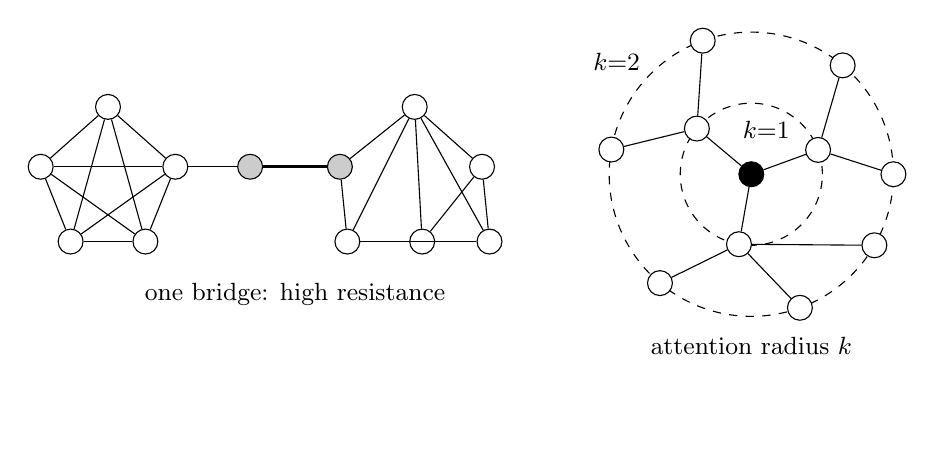
\begin{tikzpicture}[every node/.style={circle,draw,fill=white,inner sep=0pt,minimum size=9pt},scale=0.95]
  % left: two dense groups joined by one bridge edge
  \node (a1) at (0,1.2) {}; \node (a2) at (-0.9,0.4) {}; \node (a3) at (0.9,0.4) {};
  \node (a4) at (-0.5,-0.6) {}; \node (a5) at (0.5,-0.6) {};
  \foreach \x/\y in {a1/a2,a1/a3,a2/a3,a2/a4,a3/a5,a4/a5,a1/a4,a1/a5,a2/a5,a3/a4} \draw (\x) -- (\y);
  \node[fill=gray!40] (b1) at (1.9,0.4) {}; \node[fill=gray!40] (b2) at (3.1,0.4) {};
  \node (c1) at (4.1,1.2) {}; \node (c2) at (3.2,-0.6) {}; \node (c3) at (4.2,-0.6) {};
  \node (c4) at (5.0,0.4) {}; \node (c5) at (5.1,-0.6) {};
  \foreach \x/\y in {c1/c2,c1/c3,c2/c3,c1/c4,c3/c4,c3/c5,c4/c5,c2/c5,c1/c5} \draw (\x) -- (\y);
  \draw (a3) -- (b1); \draw[very thick] (b1) -- (b2); \draw (b2) -- (c1); \draw (b2) -- (c2);
  \node[draw=none,fill=none] at (2.5,-1.3) {\small one bridge: high resistance};
  % right: k-hop attention radius around a centre node
  \begin{scope}[xshift=8.6cm,yshift=0.3cm]
    \draw[dashed] (0,0) circle (0.95); \draw[dashed] (0,0) circle (1.9);
    \node[fill=black] (v) at (0,0) {};
    \foreach \ang in {20,140,260} \node (n\ang) at (\ang:0.95) {};
    \foreach \ang in {0,50,110,170,230,290,330} \node (m\ang) at (\ang:1.9) {};
    \foreach \ang in {20,140,260} \draw (v) -- (n\ang);
    \draw (n20) -- (m0); \draw (n20) -- (m50); \draw (n140) -- (m110); \draw (n140) -- (m170);
    \draw (n260) -- (m230); \draw (n260) -- (m290); \draw (n260) -- (m330);
    \node[draw=none,fill=none] at (0.2,0.6) {\small $k{=}1$};
    \node[draw=none,fill=none] at (-1.8,1.5) {\small $k{=}2$};
    \node[draw=none,fill=none] at (0,-2.3) {\small attention radius $k$};
  \end{scope}
\end{tikzpicture}
\par\smallskip
\begin{minipage}{0.95\textwidth}\small
\textit{Note.} Left: two dense groups joined by a single bridge (thick edge). Every message between the groups must cross it, so it is a bottleneck and the effective resistance between the groups is high. Right: with attention radius $k$, the black node may attend directly to every node inside the $k$-th dashed ring. The rings grow quickly with $k$: a larger radius adds shortcuts past bottlenecks but puts more nodes into each attention step.
\end{minipage}
\end{figure}

\subsubsection{Attention: A Direct Line, and Too Many Voices in the Room}
A graph transformer \citep{vaswani2017,dwivedi2021} gives every node a direct line to every other node. In each layer, node $v$ scores every node $u$ for relevance, turns the scores into weights that sum to one (a \emph{softmax}), and takes a weighted average of their states. There is no bridge to cross, so over-squashing cannot happen in the same way. The cost is \emph{dilution}. On a graph with 35,000 nodes, the weights must be shared among 35,000 candidates, most of them irrelevant. If attention does not learn to concentrate, the useful voice is drowned out by the crowd: too many voices in the room \citep{xing2024}. We measure this with \emph{attention entropy}, which is low when a node focuses on a few others and high when its attention is spread thin. Dividing by its maximum, $\log N$, gives a number between 0 (focused) and 1 (uniform).

\subsubsection{Task Range: How Far Must a Node Listen?}
Some tasks need only a node's close neighbours; others need nodes several hops away. \citet{bamberger2025} turn this into a number. For a trained model, they measure how much each input node influences each output node (again through the Jacobian), and take the influence-weighted average distance. If a node's prediction depends mostly on nodes two hops away, its range is about two. A task's range is then a property we can measure, rather than a label we assume.

\subsubsection{Why Social Graphs Are Interesting, and Hard}
Social graphs are \emph{small-world} networks \citep{f_watts1998}. Most users are only a few hops from each other: on the Higgs follow graph the effective diameter (the distance within which 90\% of pairs fall) is about 3.7 hops, and a user has about 30 follow links on average. Social graphs also have \emph{hubs}, accounts with very many links. Both facts shape the experiments. First, $k$-hop neighbourhoods grow very fast, so by three hops a node can reach most of the graph. ``Long range'' therefore means two or three hops here, not twenty. Second, on large, well-connected graphs effective resistance collapses to a simple function of degree, $R(u,v)\approx 1/d_u+1/d_v$, where $d_u$ is the number of links of node $u$ \citep{f_vonluxburg2014}. Raw resistance then mostly tells us whether the two endpoints are hubs, not whether a bottleneck lies between them. We therefore use \emph{excess resistance}, the part of $R$ left over after removing this degree term (Section~\ref{sec:measurements}).

\subsubsection{Choosing a Clean Knob: Why $\alpha$ Was Flawed and Why the Radius $k$ Is Better}
Our first design placed every model on one dial. In each layer a hybrid computes a message-passing update and an attention update and mixes them as $(1-\alpha)\cdot\mathrm{Norm}(\text{MP}) + \alpha\cdot\mathrm{Norm}(\text{Attention})$, from $\alpha=0$ (pure message passing) to $\alpha=1$ (pure attention). The problem is in the normalisation layers. They come with learnable scale parameters, so during training the model can simply turn one branch up and the other down, undoing any $\alpha$ strictly between 0 and 1. The dial then sets only the starting point of training, not the final model. We fixed this by removing the learnable scales from the two branch norms, which makes $\alpha$ a true fixed weight.

The cleaner knob is the \emph{attention radius} $k$ (Figure~\ref{fig:intuition}, right): attention may only look at nodes within $k$ hops. At $k=0$ there is no attention and the model is pure message passing; at $k=\infty$ attention covers the whole graph. A larger $k$ adds shortcuts past bottlenecks, which reduces over-squashing, but it also puts more nodes into each softmax, which increases dilution. The best $k$ is exactly the trade-off the thesis is about. Unlike $\alpha$, no learned weight can undo it, because nodes outside the radius are simply not visible. Restricting or reshaping attention by hop distance is not new \citep{f_gutteridge2023,f_abboud2022,ying2021}; our contribution is to use the radius as a diagnostic knob alongside the measurements.

\subsubsection{Planted Targets: A Known Answer}
On real labels we cannot know the true range of the task, so we cannot tell whether the range measure is right or whether the best radius tracks it. \emph{Planted} (semi-synthetic) targets solve this. We keep the real graph and the real features, add a few random input columns, and define the label from those columns so that it depends on nodes at exactly $k$ hops and on nothing closer. The ground-truth range is then $k$ by construction. This lets us check that the measured range of a trained model recovers $k$, and ask whether the best attention radius grows with $k$.

\subsubsection{How the Experiments Fit Together}
The work runs in phases S0 to S6 (Table~\ref{tab:phases} in the Methodology). In plain words: S0 asks what the social graphs look like and whether resistance means anything on them. S1 builds models that can run on graphs with tens of thousands of nodes. S2 asks whether reaching further helps on real social labels. S3 asks the same question when we know the right answer. S4 combines the results into the phase diagram. S5 asks whether pretrained graph foundation models reach far enough. S6 releases the planted tasks so others can test their models.

\subsection{Literature Review}
\textit{Over-squashing.} \citet{alon2021} showed that message-passing networks struggle when a node must summarise exponentially many distant nodes in a fixed-width vector, and named the effect over-squashing. \citet{topping2022} tied it to negatively curved edges and proposed rewiring the graph. \citet{digiovanni2023} bounded the Jacobian sensitivity between two nodes in terms of width, depth and graph topology, and \citet{black2023} showed that total effective resistance bounds over-squashing, which makes resistance a structural predictor that can be computed before training. \citet{mishayev2025} argued that over-squashing can arise even between nearby nodes. These results describe what a model class \emph{can} do; we measure what trained models \emph{do}. For large graphs, \citet{f_vonluxburg2014} proved that resistance converges to $1/d_u+1/d_v$, which is why we correct for degree.

\textit{Graph transformers and reach.} Early graph transformers added Laplacian positional encodings to attention \citep{dwivedi2021}. Graphormer biased attention by shortest-path distance \citep{ying2021}, and spectral attention made the encodings learnable \citep{kreuzer2021}. GPS combined a message-passing layer and a global attention layer in every block \citep{rampasek2022}. Exphormer \citep{shirzad2023} and the Performer \citep{f_choromanski2021} reduce the quadratic cost of attention, the latter with random features that give linear cost; we use the Performer for full-graph attention. Between the two extremes, DRew lets nodes connect to $k$-hop neighbours gradually as depth grows \citep{f_gutteridge2023}, and Shortest Path Networks aggregate separately over each hop distance \citep{f_abboud2022}. Our radius knob sits in this family.

\textit{Dilution.} In language models, accuracy drops when relevant content sits in the middle of a long context \citep{liu2024}. In graphs, \citet{xing2024} described over-globalizing, where global attention puts weight on distant, irrelevant nodes and hurts accuracy, and \citet{sun2025} linked a similar over-aggregation effect to the number of nodes attention covers. Gated and capacity-controlled global attention has been proposed as a remedy \citep{liu2026}.

\textit{Measuring range, and benchmarks.} The Long Range Graph Benchmark was designed to need long-range interactions \citep{dwivedi2022}, but \citet{tonshoff2024} showed that tuned message-passing baselines close most of the gap, and \citet{bamberger2025} found with their range measure that models on its Peptides tasks use mostly short-range information. ECHO \citep{miglior2025} builds tasks with controlled long-range dependencies, on synthetic graphs and molecules. Neither benchmark contains social graphs, and in social graphs ``far'' means a few hops through very large neighbourhoods, a different regime from long chains.

\textit{Graph foundation models.} \citet{f_gutteridge2026} showed that foundation models with a fixed message-passing backbone under-reach on tasks whose range differs from their training tasks. GraphPFN \citep{f_eremeev2026} is a node-level foundation model pretrained on synthetic graphs that uses attention to aggregate over neighbourhoods. NodeGround \citep{f_lee2026} found that tuned GNNs still beat foundation models overall on node classification, but did not analyse range. Testing an attention-based foundation model on planted-range social tasks extends both lines of work.

\textit{Social graph data.} We use SNAP data \citep{f_leskovec2014}: the Reddit hyperlink network \citep{kumar2018}, the Twitch networks \citep{f_rozemberczki2021,f_rozemberczki2021b}, and the Twitter activity around the 2012 Higgs boson announcement \citep{f_dedomenico2013}.

% ================================================================
\section{Data}
All main experiments use four public social graphs from SNAP \citep{f_leskovec2014} (Table~\ref{tab:datasets}). We treat every graph as undirected for message passing and for distances. Each dataset has one real target, chosen so that it is not trivially predicted from a node's own features. On top of these real targets we add planted targets (Methodology).

\begin{table}[htbp]
\caption{Social graphs and real targets}
\label{tab:datasets}
\centering\small
\begin{tabular}{@{}L{1.0in}L{1.3in}L{2.0in}L{0.55in}L{0.85in}@{}}
\toprule
Dataset & Graph & Target & Metric & Subgraphs (train/val/test) \\
\midrule
twitch-gamers & 168,114 users, 6.8M mutual-follow edges & \texttt{mature}: channel marked as explicit content (binary, about 47\% positive) & AUROC & 58/13/13 (2k nodes) \\
twitch-de & 9,498 users, 153,138 edges & \texttt{mature} (binary) & AUROC & 13/3/3 (500 nodes) \\
reddit-body & 35,776 subreddits, 124,330 undirected links & \texttt{LIWC\_Money}: share of money-related words in a community's posts (regression) & $R^2$ & 12/3/3 (2k nodes) \\
higgs-follow & 35,593 users, 528,532 follow edges & \texttt{active\_after}: user retweets, mentions or replies after the cutoff (binary, about 47\% positive) & AUROC & 12/3/3 (2k) or 49/11/11 (500) \\
\bottomrule
\end{tabular}
\par\smallskip
\begin{minipage}{0.95\textwidth}\small
\textit{Note.} Subgraphs are METIS parts; in full-graph mode the same parts only decide which nodes are labelled in each split (Methodology). The Higgs graph has a second target, \texttt{activate\_passive}, described below.
\end{minipage}
\end{table}

\subsection{Data Sources}
\textit{Twitch gamers} \citep{f_rozemberczki2021b}. Nodes are Twitch users and edges are mutual follows. Each user has account fields: views, account lifetime, creation and update dates, language, and flags for affiliate status and dead accounts. The target is the \texttt{mature} flag, whether a channel is marked as explicit content. Views are log-scaled and language is one-hot encoded.

\textit{Twitch German network} \citep{f_rozemberczki2021}. A smaller, denser Twitch graph of German-language streamers. Inputs are the games a user plays, reduced to the 128 most common games, plus account fields (days active, partner status, log views). The target is again \texttt{mature}.

\textit{Reddit hyperlinks} \citep{kumar2018}. Nodes are subreddits (communities). An edge records a post in one subreddit that links to another; there are 286,561 such directed links, which give 124,330 undirected edges. Each post carries 86 numeric properties (text length, sentiment and LIWC word-category scores), and a subreddit's features are the averages over its outgoing posts. Subreddits with no outgoing posts have no features; they relay messages but are never scored. To pick a target that depends on the neighbourhood, we ranked candidate columns by how much a ridge regression improved when a node's own features were joined by the average features of its 1- to 4-hop neighbourhoods. \texttt{LIWC\_Money} ranked first: $R^2$ rose from 0.108 with own features to 0.185 with four hops. Input columns that correlate above 0.9 with the target are removed so the model cannot copy it.

\textit{Twitter Higgs} \citep{f_dedomenico2013}. This dataset records Twitter activity around the announcement of the Higgs boson discovery in July 2012: who follows whom, and timestamped retweets, mentions and replies. The target \texttt{active\_after} asks: will this user retweet, mention or reply to anyone after the cutoff, 4 July 2012 00:00 UTC (a few hours before the announcement)? It is a social-influence question: does the activity of the people you follow predict whether you join the conversation? The second target, \texttt{activate\_passive}, is the same label scored only on the roughly 11\% of users who had no activity before the cutoff. Their own history says nothing, so any signal must come from their neighbours.

\textit{Leakage controls for Higgs.} A predictive model must not see the future. We enforce three rules. (1) The node set is users involved in at least one interaction \emph{before} the cutoff; SNAP's full user set includes users who appear only because of later activity, which would leak the label through the node set itself. (2) The graph is the follow graph on that node set. The activity layers (retweet, reply, mention) are rebuilt from timestamped records before the cutoff only; SNAP's ready-made layers cover the whole week and are never used. (3) The inputs are follow in- and out-degree and, for each activity type, the pre-cutoff out-count, in-count and number of distinct partners. A check at build time asserts that every record used for inputs or layers is dated before the cutoff. One channel remains: SNAP does not say when the follow graph was collected, so follow links formed after the cutoff cannot be excluded.

\subsection{Descriptive Analysis}
Table~\ref{tab:structure} summarises the structure of the test subgraphs. Three properties shape the analysis.

\begin{table}[htbp]
\caption{Structure of the social graphs (mean over test subgraphs)}
\label{tab:structure}
\centering\small
\begin{tabular}{@{}lcccc@{}}
\toprule
Dataset & Mean degree & Effective diameter & Mean excess resistance & Spearman $\rho$ \\
\midrule
twitch-gamers & 11.6 & 5.8 & 0.39 & 0.90 \\
reddit-body   & 4.3  & 5.7 & 0.49 & 0.77 \\
twitch-de     & 22.9 & 3.0 & 0.02 & 0.998 \\
higgs-follow  & 16.7 & 3.7 & 0.09 & 0.98 \\
\bottomrule
\end{tabular}
\par\smallskip
\begin{minipage}{0.95\textwidth}\small
\textit{Note.} Effective diameter is the hop distance within which 90\% of node pairs fall. Excess resistance is $R(u,v)-(1/d_u+1/d_v)$ (Section~\ref{sec:measurements}). The last column is the Spearman rank correlation between resistance $R$ and its degree-only limit $1/d_u+1/d_v$; values near one mean resistance mostly measures degree.
\end{minipage}
\end{table}

First, the graphs are small-world. Effective diameters range from 3.0 to 5.8 hops inside the subgraphs, so a few hops cover most nodes. Planted ranges larger than three or four hops are therefore not meaningful on these graphs.

Second, raw resistance mostly restates degree. Its rank correlation with $1/d_u+1/d_v$ is 0.90 or higher on three of the four graphs and 0.77 on Reddit. Only the sparse Higgs retweet layer breaks the pattern (correlation 0.07), and that layer is too sparse to use. Excess resistance keeps the part that degree does not explain. It is largest on Reddit and Twitch gamers, which are the sparser graphs, and close to zero on the dense Twitch German graph. The graphs therefore cover a range of bottleneck levels, which the phase diagram needs.

Third, the Higgs activity layers before the cutoff are very sparse, with mean degree 1.4 for retweets and 0.16 for replies. We had planned to compare the same users under two different graph structures (follow versus reply), but these layers are too thin to train on, so all Higgs experiments use the follow graph.

Finally, partitioning cuts many edges. On Twitch gamers only 26\% of edges fall inside the 2,000-node parts, and on Higgs-follow 32\% of edges fall inside 500-node parts and 47\% inside 2,000-node parts. In a small-world graph, any way of cutting it into pieces removes many links, which turned out to matter (Methodology, Training and Evaluation).

% ================================================================
\section{Methodology}
The methodology follows three principles. Comparisons change one knob at a time, because every graph model is built from the same layer. Mechanisms are measured directly on trained models, not only inferred from accuracy. And each claim is checked against a case where we know the answer, either an analytic test case or a planted target. All code is a tested Python package, \texttt{gnn\_mech}; earlier versions of the pipeline are described in Appendix~\ref{app:background}.

\subsection{Feature Engineering and Leakage Controls}
The pipeline has four steps. (1) Download and parse each SNAP source into one cached graph. (2) Build node inputs and the target from the raw node table, with the Higgs leakage rules above. Skewed counts are log-scaled, and every input column is standardised with statistics from the training-labelled nodes only. Regression targets are standardised the same way. (3) Partition the graph with METIS \citep{f_karypis1998}, a standard tool that cuts a graph into parts of roughly equal size with few edges between them. Whole parts are assigned to training, validation and test (70/15/15 of the parts), using a \emph{split seed}. Because parts, not single nodes, are assigned, each split's labelled nodes form connected regions, which is closer to predicting for a new region of the network than random node sampling. (4) Optionally add a random-walk positional encoding (the probability that a random walk returns to its start after $1,\dots,16$ steps), which helps attention know where a node sits. It is used on subgraphs; full-graph runs do not use it.

\textit{The partitions decide which nodes are labelled.} This is the key leakage control. A node's label is used for training only if its part is in the training split; validation and test labels are never used in the loss or for scaling. Nodes in other splits may still appear as unlabelled inputs in full-graph mode (below), as in standard transductive node classification \citep{kipf2017}.

\subsection{Planted Targets with a Known Range}
Planted targets keep the real graph and real features (now nuisance inputs) and append a few random input columns. The label is an exact function of the planted columns on the graph, so its range is known. Let $S_k(v)$ be the \emph{shell} of nodes exactly $k$ hops from $v$, computed on the full graph. We use two families.

\textit{Shell mean} (a sanity check). Each node gets one random value $z_u\sim\mathcal N(0,1)$, and the label is the average of $z$ over the $k$-hop shell, $y_v=\frac{1}{|S_k(v)|}\sum_{u\in S_k(v)} z_u$. This tests pure reach: a model must gather values from exactly $k$ hops away. It has a known loophole on small-world graphs: when the shell is almost ``everything at distance $k$ or more'', the label can be inferred from the inner nodes, because the total over the graph is fixed. We record how well this shortcut predicts the label.

\textit{Retrieve} (the main test). Every node $u$ carries a key, one of $K$ discrete codes shown to the model as a random vector, and a value $w_u\sim\mathcal N(0,1)$. Node $v$ carries a query code. The query is chosen to match the key of a random node in $v$'s $k$-hop shell, and no node closer than $k$ hops carries that key. The label is the value of the matching shell node (the average, if several shell nodes share the key). The task is like asking a friend-of-a-friend-of-a-friend a question: the node must find the one distant node whose key matches its query and fetch its value. Nothing closer carries any information about the answer, so the range is exactly $k$. Nodes farther than $k$ hops may also carry the key; they are distractors that a model with unlimited reach must learn to ignore. Because shells grow very fast on social graphs, the number of key codes $K$ is set separately for each $k$ (from the 90th percentile of the $k$-hop neighbourhood sizes), so that the expected number of extra matches stays below one for most nodes.

Nodes without a valid target (an empty shell, or no eligible query) are left unlabelled. Targets are deterministic given the graph, family, $k$ and a seed. For both families we compute the range of the target function itself from its exact Jacobian; it equals $k$ by construction, and a unit test checks this. On Higgs-follow we use $k\in\{1,2,3,4\}$. Shell sizes and eligible nodes per $k$ on Higgs-follow are reported in the Findings.

\subsection{Modeling Framework}

\subsubsection{The Hybrid Layer}
Every graph model except the GCN baseline is a stack of the same layer. Given node states $x$ and edges $E$, one layer computes
\begin{align*}
h_{\text{loc}} &= \mathrm{BN}_{\text{loc}}\big(\mathrm{Local}(x,E)\big), \qquad
h_{\text{att}} = \mathrm{BN}_{\text{att}}\big(\mathrm{Attn}(x)\big),\\
x' &= x + \mathrm{Dropout}\big((1-\alpha)\,h_{\text{loc}} + \alpha\,h_{\text{att}}\big),\qquad
x'' = \mathrm{BN}_{\text{ffn}}\big(x' + \mathrm{FFN}(x')\big),
\end{align*}
where BN is batch normalisation \citep{f_ioffe2015} and FFN is a small two-layer network applied to each node. When $\alpha=0$ the attention branch is not built and the model is a pure message-passing network (MPNN); when $\alpha=1$ the local branch is not built and the model is a pure transformer. A prediction head maps each node's final state to its output.

\textit{Local branch.} We use a GCN-normalised message-passing step \citep{kipf2017}: each node averages its neighbours' states, weighting each neighbour by $1/\sqrt{d_u d_v}$, then applies a linear map. Our first sweep used GINE \citep{hu2020}, which sums neighbour messages; on social graphs the sum over a hub's hundreds of neighbours gave large, unstable messages, so we switched to the degree-normalised version.

\textit{Affine-free branch norms.} With the default learnable scale and shift in $\mathrm{BN}_{\text{loc}}$ and $\mathrm{BN}_{\text{att}}$, training can rescale either branch and cancel $\alpha$ (Background). We set these two norms to have no learnable parameters, so $\alpha$ is a true fixed weight. The feed-forward norm keeps its parameters, since it does not affect the mix.

\subsubsection{Attention Variants}
\textit{Softmax attention} is standard multi-head self-attention \citep{vaswani2017} over all nodes of a subgraph. Its cost grows with the square of the number of nodes, which is fine for 500-node subgraphs.

\textit{Performer attention} \citep{f_choromanski2021} approximates softmax attention with random features, so its cost grows linearly with the number of nodes. We use it for full attention ($k=\infty$) on the full 35,593-node Higgs graph, with 64 random features per head. In evaluation the random features are fixed, so measurements are repeatable.

\textit{Radius attention} is softmax attention in which node $v$ may attend only to nodes within $k$ hops. On small subgraphs it masks the dense attention matrix. On the full graph it works on a precomputed list of all node pairs within $k$ hops, with a cap on the number of pairs to bound memory. On the Higgs follow graph there are 1.09 million pairs within one hop but 298.8 million within two, so only radius 0, 1 and $\infty$ fit on a single GPU there.

\subsubsection{Model Variants and Baselines}
Table~\ref{tab:variants} lists the variants. Both knobs live in the same layer. In the $\alpha$ sweep the attention covers the whole (sub)graph and $\alpha$ varies. In the radius sweep $\alpha$ is fixed at 0.5 and the radius $k$ varies; $k=0$ means no attention ($\alpha=0$).

\begin{table}[htbp]
\caption{Model variants}
\label{tab:variants}
\centering\small
\begin{tabular}{@{}L{1.6in}L{4.4in}@{}}
\toprule
Variant & Description \\
\midrule
MLP & No graph: each node is predicted from its own features only. The yardstick for any graph effect. \\
GCN & A plain graph convolutional network \citep{kipf2017} with residual connections, in the style of the tuned baselines of \citet{tonshoff2024}; same depth and width as the other models. \\
Hybrid, $\alpha\in\{0,.25,.5,.75,1\}$ & The layer above with full attention (softmax on subgraphs, Performer on the full graph). $\alpha=0$ is the MPNN, $\alpha=1$ the transformer. \\
Radius, $k\in\{0,1,2,\infty\}$ & The layer above with $\alpha=0.5$ and attention limited to $k$ hops. \\
\bottomrule
\end{tabular}
\end{table}

Unless stated otherwise, models have four layers, hidden width 64, four attention heads and dropout 0.1.

\subsection{Training and Evaluation}
\textit{Subgraph training.} In our first design, each METIS part was a separate small graph: message passing and attention ran only inside the part, and a batch held eight parts. This is the usual way to train on graphs too large for memory, and it keeps the splits fully separate. It turned out to be a poor fit for social graphs. On Higgs-follow only 32\% of follow edges stay inside 500-node parts, and a logistic-regression check showed that the neighbour signal available with full-graph neighbours largely disappears with in-part neighbours (details in the Findings). Subgraph training throws away the edges the knobs are meant to probe, and planted $k$-hop targets would suffer even more, since their shells cross part boundaries.

\textit{Full-graph (transductive) training.} Our main setup therefore keeps the whole graph. The METIS parts only decide which nodes are labelled for training, validation and test. Message passing and attention use all 35,593 Higgs nodes and all their edges in every split; only the loss and the scores are restricted to the split's labelled nodes. Every step processes the whole graph, so there is one optimiser step per epoch, and runs use several hundred epochs with a long early-stopping patience. Subgraph runs use up to 100 epochs with patience 20.

\textit{Optimisation.} All models use AdamW \citep{loshchilov2019} with learning rate $10^{-3}$, five warm-up epochs then cosine decay, and gradient clipping at 1.0. Binary targets use cross-entropy loss and regression targets use squared error. We keep the checkpoint with the best validation score.

\textit{Metrics.} For binary targets we report the area under the ROC curve (AUROC): the probability that a randomly chosen positive node is scored above a randomly chosen negative one. It is 0.5 for random guessing and 1 for a perfect ranking, and it does not depend on a threshold. We also record average precision. For regression targets (Reddit and the planted targets) we report $R^2$, the share of the target's variance the model explains: 0 for predicting the mean, 1 for a perfect fit.

\textit{Seeds.} Two kinds of randomness are separated. The \emph{split seed} decides the METIS partition and which parts are training, validation and test. The \emph{model seed} decides weight initialisation and dropout. On Higgs we use three split seeds and two model seeds per variant (six runs), and report the mean and standard deviation over runs; the first sweep used three model seeds on one split. Planted-target runs use one split seed and two model seeds. All choices of $\alpha$ and $k$ are made on validation data.

\subsection{Mechanistic Measurements}
\label{sec:measurements}
All measurements use the best checkpoint in evaluation mode. Each was first checked on cases with a known answer: resistance equals hop distance on a path; uniform attention gives normalised entropy one; a model that reads exactly the $d$-hop neighbour has range $d$.

\textit{Effective resistance and excess resistance.} With $L$ the graph Laplacian and $L^{+}$ its pseudo-inverse, $R(u,v)=(e_u-e_v)^\top L^{+}(e_u-e_v)$, where $e_u$ is the indicator vector of node $u$. It is computed exactly on graphs of up to 5,000 nodes and approximately above that. Because $R$ tends to $1/d_u+1/d_v$ on large graphs \citep{f_vonluxburg2014}, we report the excess resistance
\[
\tilde R(u,v) = R(u,v) - \Big(\frac{1}{d_u}+\frac{1}{d_v}\Big),
\]
the resistance left over after the degree term. High excess resistance means a bottleneck beyond what the endpoints' degrees explain.

\textit{Jacobian sensitivity.} $J(u,v)=\lVert\partial h_v/\partial x_u\rVert$, the size of the change in node $v$'s final state for a small change in node $u$'s input. For sampled target nodes $v$, one backward pass gives the sensitivity to every source $u$. We relate $\log J$ to hop distance, raw resistance and excess resistance. A steeper fall with excess resistance means stronger over-squashing.

\textit{Attention entropy.} For an attention layer and head, node $i$'s attention weights $a_{ij}$ over the $N_i$ nodes it can see have entropy $-\sum_j a_{ij}\log a_{ij}$. Dividing by $\log N_i$ gives a value in $[0,1]$: near 0 when focused, near 1 when spread evenly. It is computed per head, since averaging heads first would inflate it. For softmax and radius attention the weights are exact. The Performer has no explicit attention matrix, but the row for a single query node can be computed exactly from its random features, so we compute entropy on sampled query nodes.

\textit{Range.} Following \citet{bamberger2025}, the influence of source $u$ on target $v$ is $I_{vu}=\sum\lvert\partial y_v/\partial x_u\rvert$ (summed over input channels), and the range of $v$ is the influence-weighted mean distance
\[
\rho_v=\frac{\sum_u I_{vu}\,d(v,u)}{\sum_u I_{vu}},
\]
with $d$ the hop distance (or resistance). On planted targets we compare the measured range of each trained model with the planted $k$; a correct measure should rise with $k$.

\subsection{Experimental Plan}
Table~\ref{tab:phases} lists the phases, the question each answers and its status on 3 November 2026.

\begin{table}[htbp]
\caption{Experimental phases and status}
\label{tab:phases}
\centering\small
\begin{tabular}{@{}L{0.35in}L{2.35in}L{2.3in}L{0.95in}@{}}
\toprule
Phase & Question in plain words & Design & Status \\
\midrule
S0 & What do the social graphs look like, and does resistance mean anything on them? & Loaders, partitions, structure statistics, excess resistance & Done \\
S1 & Can we run attention on graphs with tens of thousands of nodes? & Performer and radius attention, node-level models, MLP and GCN baselines & Done \\
S2 & Does reaching further help on real social labels? & $\alpha$ and radius sweeps on real targets, on subgraphs and on the full graph, with all measurements & In progress \\
S3 & Does the best reach follow the task's range when we know it? & Planted shell-mean and retrieve targets, $k=1$--4, on Higgs & Being built \\
S4 & Can structure and range predict the best setting? & Phase diagram: excess resistance $\times$ task range, coloured by the best knob setting & Planned \\
S5 & Do graph foundation models reach far enough? & GraphPFN (and possibly GraphAny) on the planted tasks; measure their range & Planned \\
S6 & Can others test their models on the same tasks? & Release generator code, node indices and seeds (no raw data) & Planned \\
\bottomrule
\end{tabular}
\end{table}

A radius sweep on 500-node subgraphs has finished and is reported in the Findings as a control. The running experiments are: (1) the full-graph $\alpha$ sweep and radius sweep on Higgs, for both targets, with three split seeds and two model seeds; and (2) the planted-target sweep on the full Higgs graph, with $k\in\{1,2,3\}$, both families and the variants MLP, GCN, MPNN ($\alpha=0$), full attention ($\alpha=1$), hybrid ($\alpha=0.5$) and radius 1 (radius 2 does not fit in memory on this graph). \pending{Full-graph $\alpha$ and radius sweep results} \pending{Planted-target sweep results and measured range versus planted $k$}

Two scale limits apply. Small-world structure means that $k\ge3$ covers most of the Higgs graph, so radius values beyond two are close to full attention, and planted ranges beyond four are not meaningful. And full-graph training needs the whole graph in GPU memory, which limits width and the number of attention pairs. The other datasets will move to full-graph or large-subgraph setups after Higgs.
